\documentclass[dvipdfmx, twocolumn, a4paper]{hcresume}

\usepackage{epsfig}
\usepackage{amsmath}
\usepackage{graphics}
\usepackage{graphicx}
\usepackage{txfonts}
\usepackage{color}
\usepackage{BoldGothic4fig}
\usepackage{bm}
\usepackage{verbatim}
\usepackage{wrapfig}
\usepackage{ascmac}
\usepackage{makeidx}
\usepackage{enumerate}
\usepackage{comment}
\usepackage{multirow}
\usepackage{listings}

\usepackage[hang,small,bf]{caption}
\usepackage[subrefformat=parens]{subcaption}

%
\def\linesparpage#1{\baselineskip=\textheight
   \divide\baselineskip by #1}
\def\kcharparline#1{%
   \ifx\xkanjiskip\undefined%
   \jintercharskip 0mm plus 0.2mm minus 0.2mm
   \else
   \xkanjiskip 0mm plus 0.2mm minus 0.2mm
   \fi
   \settowidth{\textwidth}{}%
   \multiply\textwidth by #1}
%
\newcommand\figref[1]{\textbf{図~\ref{fig:#1}}}
\newcommand\tabref[1]{\textbf{表~\ref{tab:#1}}}
\newcommand{\bhline}[1]{\noalign{\hrule height #1}}

\hcheader{MIプログラム 卒研中間発表会}
\title{\bf 評価者特性の時間変動を考慮した項目反応モデル}
\author{1810519 林真由}
\supervisor{指導教員 宇都 雅輝 准教授}

\begin{document}
\maketitle
\pagestyle{empty}
\thispagestyle{empty}
\section{はじめに}
近年,大学入試や資格試験,教育評価などにおいて,パフォーマンス評価のニーズが高まっている.一方で,パフォーマンス評価では,多肢選択式試験のような客観的評価と異なり人間の評価者が採点を行うため,評価者の厳しさや一貫性などの特性差により,採点に偏りが生じ,受検者の能力測定の信頼性が低下する問題が知られている.このような問題を解決する数理的なアプローチの一つとして,評価者の特性を考慮した項目反応理論(Item response theory:IRT)\cite{IRTLord}が近年注目されている.

それらのモデルでは,評価者の特性差の影響を考慮した能力推定を行うことができる.一方で,既存モデルのほとんどは評価者の特性が評価中に変化しないことを仮定している.しかし,多数の受験者を長時間かけて採点するような場合には,この仮定は成り立たないことがある.評価者の特性が採点の過程で変化する現象は評価者ドリフト(Rater Drift)と呼ばれ,これを考慮したモデルも提案されている.具体的には,一定の時間区分ごとの評価者の厳しさパラメータを導入することで,評価者特性の時間変化を捉えるモデルとなっている.しかし,このモデルでは各時間区分ごとのパラメータが独立しているため,パラメータの推定が不安定となり,評価者特性の時間変化の解釈が難しくなる問題がある.

この問題を解決するため,本研究では,時間区分ごとの評価者の厳しさパラメータにマルコフ性を仮定した新しい項目反応モデルを提案する.提案モデルでは,既存モデルよりも安定したパラメータ推定が可能となり,モデルの性能が改善すると考えられる.本研究では,シミュレーション実験と実データ実験を通して提案モデルの有効性を示す.

\section{項目反応理論}
本研究では,高精度な能力推定を行うために,IRTを利用する.

現在,評価者特性を最も柔軟に表現できる項目反応モデルとして,一般化多相ラッシュモデルが知られている\cite{g-MFRM}.
このモデルでは,評価者$r$が課題$i$における受検者$j$のパフォーマンスにスコア$k$を与える確率を次式で定義する.
\begin{displaymath}
  P_{ijrk}=\frac{\mathrm{exp}\sum_{m=1}^{k}\{\alpha_i\alpha_r(\theta_{j}-(\beta_{i}+\beta_{r})-d_{rm})\}}{\sum_{l=1}^{K}\mathrm{exp}\sum_{m=1}^{l}\{\alpha_i\alpha_r(\theta_{j}-(\beta_{i}+\beta_{r})-d_{rm})\}}
\end{displaymath}
ここで,$\alpha_i$は課題$i$の識別力,$\alpha_r$は評価者$r$の一貫性,$\theta_j$は受検者$j$の能力,$\beta_i$は課題$i$の困難度,$\beta_r$は評価者$r$の厳しさ,$d_{rk}$は評価者$r$のスコア$k$に対する厳しさを表すステップパラメータである.モデルの識別性のために,$\sum^{I}_{i=1}{\mathrm{log}\alpha_i}=0$,$\sum^{I}_{i=1}{\beta_i}=0$,$\sum^{K}_{k=2}{d_{rk}}=0$,$d_{r1}=0$を仮定する.
なお,以降で紹介する評価者ドリフトを考慮したモデルや提案モデルでは,課題数が1の場合を想定し,課題パラメータは考慮しないこととする.

上記のモデルは評価者の特性が評価中に変化しないことを仮定しているが,この仮定は現実には成り立たないことがある.
このような評価者ドリフトを考慮できるモデルとして,時間区分$t$における評価者$r$の厳しさの変化を反映させるモデルが提案されている\cite{Raudenbush}.このモデルでは,評価者$r$が時間区分$t$で採点した受検者$j$のパフォーマンスに,スコア$k$を与える確率を次式で表す.
\begin{displaymath}
  P_{jrtk}=\frac{\mathrm{exp}\sum_{m=1}^{k}(\theta_{j}-\beta_{r} - \pi_{r}\beta_{rt}-d_{m})}{\sum_{l=1}^{K}\mathrm{exp}\sum_{m=1}^{l}(\theta_{j}-\beta_{r} - \pi_{r}\beta_{rt}-d_{m})}
\end{displaymath}
ここで,$\beta_{r}$は評価者$r$の初期の厳しさ,$\pi_{r}$は評価者$r$の厳しさの変化の傾き,$\beta_{rt}$は評価者$r$の時間区分$t$における厳しさを表す.

このモデルは,一連の採点データを一定の時間区分で区切り,時間区分ごとの評価者パラメータ$\beta_{rt}$を導入している点が特徴である.具体的には,図\ref{timeid}のように,評価者が採点した順に受検者を並べ,データ全体をいくつかの時間区分数に分割し,時間区分を表すインデックス(以降ではTimeIDと呼ぶ)を各データに付与した上で,各評価者の厳しさパラメータをTimeIDごとに推定する.

\begin{figure}[t]
  \centering
  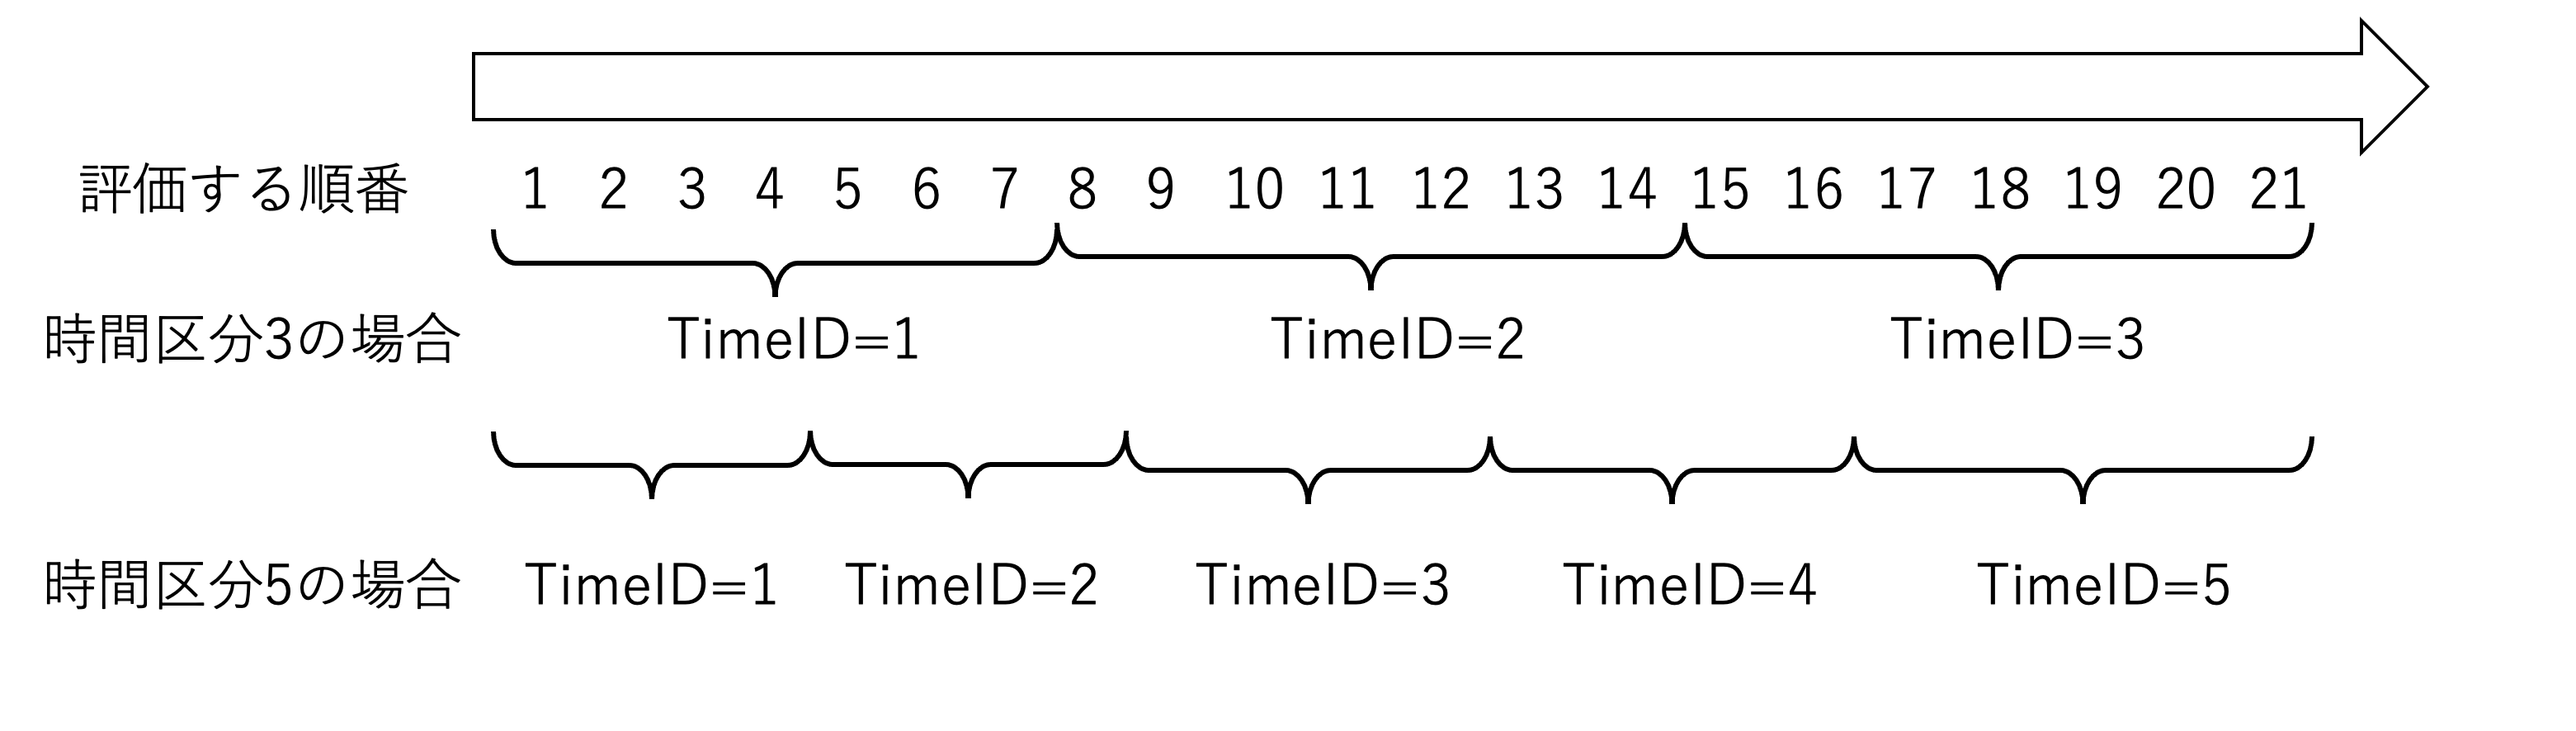
\includegraphics[width=8cm]{img/timeid.png}
  \caption{時間区分データのイメージと例}
  \label{timeid}
\end{figure}

このモデルでは,時間区分ごとの評価者特性を分析することが可能である.しかし,このモデルでは時間区分ごとのパラメータが独立していると仮定しているため,パラメータの推定が不安定となり,評価者特性の時間変化について解釈が難しくなる問題がある.
この問題を解決するため,時間区分ごとの評価者の厳しさパラメータにマルコフ性を仮定した新しい項目反応モデルを提案する.
\section{提案モデル}
提案モデルでは,評価者$r$が時間区分$t$で採点した受検者$j$のパフォーマンスに,スコア$k$を与える確率$P_{jrtk}$を次式で定義する.
\begin{displaymath}
  P_{jrtk}=\frac{\mathrm{exp}\sum^k_{m=1}{\alpha_r(\theta_{j}-\beta_{rt}-d_{rm})}}{\sum^K_{l=1} \mathrm{exp}\sum^l_{m=1}{\alpha_r(\theta_{j}-\beta_{rt}-d_{rm})}}
\end{displaymath}
\begin{eqnarray}
  \beta_{rt}\sim \mathrm{N}(\beta_{r(t-1)},\sigma)\nonumber\\
  \beta_{r1} \sim \mathrm{N}(0,1)\nonumber\\
  \sigma \sim \mathrm{LN}(-3,0)\nonumber
\end{eqnarray}

ここで,$N(\mu,\sigma^2)$は平均$\mu$,標準偏差$\sigma^2$の正規分布,$LN(\mu,\sigma^2)$は平均$\mu$,標準偏差$\sigma^2$の対数正規分布を表す.

提案モデルでは,$\beta_{rt}$が$\beta_{(r-1)t}$に依存して決まると仮定している点が特徴である.また,提案モデルでは,より柔軟に評価特性を表現するために,一般化多相ラッシュモデルでも採用されている評価者の一貫性パラメータ$\alpha_r$と各スコアに対する厳しさパラメータ$d_{rk}$も導入している.

なお,提案モデルにおける$\beta_{rt}$の事前分布のパラメータである$\sigma$は,できる限り小さい値とすることで,$\beta_{rt}(t>1)$の事後分布が縮小するため,パラメータ推定が安定すると期待できる.この事前知識に合わせて,ここでは,$\mathrm{LN}(-3,0)$を$\sigma$の事前分布として採用した.

また,提案モデルではモデルの識別性のために,$\theta_{j}\sim N(0,1)$,$\prod_{r}\alpha_r=1$, $d_{r1}=0$, $\sum_{k=2}^{K}d_{rk}=0$を仮定する.

提案モデルのパラメータ推定手法にはマルコフ連鎖モンテカルロ法(Markov chain Monte Carlo methods:MCMC)を用いる.パラメータの事前分布は$\theta_{j}$, $d_{rk}$, $\mathrm{log}\alpha_{r}$, $\beta_{rt}\sim N(0,1^{2})$とした.本研究では,MCMCのバーンイン期間は1000とし,1000$\sim$2000時点までの1000サンプルを用いる.
\section{シミュレーション実験}

本節では,MCMCによる提案モデルのパラメータ推定精度をシミュレーション実験により評価する.実験手順は以下の通りである.
(1)パラメータの真値を,前節に記載したパラメータの分布に従って生成する.
(2)手順(1)で生成したパラメータを用いて,提案モデルに従ってデータを生成する.
(3)手順(2)で生成したデータからMCMCを用いてパラメータ推定を行う.
(4)手順(3)で得られたパラメータ推定値と手順(1)で生成したパラメータ真値において,RMSE(Root Mean Square Error)とバイアスを求める.
(5)以上を5回繰り返し実行し,RMSEとバイアスの平均値を求める.

上記の実験を,受検者数$J=$50,100,評価者数$R=$10,15,時間区分数$T=$3,5,10の場合において行った.得点の段階数は$K=$5とした.
実験結果を表\ref{parameters_recovery}に示す.

\begin{table}[t]
  \begin{minipage}[t]{8cm}
    \centering
    \caption{パラメータ・リカバリ実験の結果}
    \setlength{\tabcolsep}{5.pt}
    \scalebox{0.8}{
      \begin{tabular}{cccccccccccccc}  
        \bhline{1pt}
        \multirow{2}{*}{$J$} & \multirow{2}{*}{$R$} & \multirow{2}{*}{$T$}  && \multicolumn{4}{c}{RMSE} &&   \multicolumn{4}{c}{BIAS}  \\
        \cline{5-8}\cline{10-13}
          & & & & $\theta$ & $\alpha_r$ & $\beta_{rt}$ & $d_{rk}$ &  & $\theta$ & $\alpha_r$ & $\beta_{rt}$ & $d_{rk}$ \\
        \bhline{1pt}
        50 & 10 & 3 & & 0.24 & 0.27 & 0.20 & 0.40 & &0.02  & 0.02 & 0.06  & 0.00 \\
          &   & 5  && 0.30 & 0.24 & 0.31 & 0.38 & &-0.01 & -0.00 & -0.03 & -0.00  \\
          &   & 10 && 0.32 & 0.36 & 0.36 & 0.41 && 0.01  & 0.04 & -0.02 & 0.00 \\
        \cline{2-14}
        & 15 & 3  && 0.25 & 0.30 & 0.25 & 0.37 && 0.03 & 0.01 & 0.06 & 0.00  \\
        &  & 5  && 0.25 & 0.23 & 0.19 & 0.34 && 0.03 & 0.01 & 0.01 & -0.00  \\
        &  & 10 && 0.24 & 0.26 & 0.33 & 0.39 && 0.02 & 0.02 & 0.03 & 0.00 \\
        \hline
        100 & 10 & 3  && 0.26 & 0.19 & 0.13 & 0.28 && -0.02 & 0.00 & -0.01 & 0.00  \\
        &  & 5  && 0.27 & 0.19 & 0.13 & 0.27 && 0.01  & 0.00 & 0.00  & 0.00  \\
        &  & 10 && 0.26 & 0.18 & 0.19 & 0.30 && -0.02 & 0.02 & -0.03 & -0.00 \\
        \cline{2-14}
        & 15 & 3  && 0.23 & 0.22 & 0.20 & 0.30 && 0.00 & 0.02 & 0.00 &0.00 \\
        &  & 5  && 0.23 & 0.20 & 0.18 & 0.31 && 0.03 & 0.01 & 0.06  &0.00\\
        &  & 10 && 0.24 & 0.25 & 0.40 & 0.38 && 0.01 & 0.02 & -0.01 &0.00\\
        \hline
        \multicolumn{4}{c}{Avg.}   &  0.26 & 0.24 & 0.24 & 0.34 &  & 0.01 & 0.01 & 0.01 & 0.00 & \\
        \bhline{1pt}
      \end{tabular}
    }
    \label{parameters_recovery}
  \end{minipage}
\end{table}

表\ref{parameters_recovery}から,先行研究と同様に,受検者数・評価者数の増加に伴い推定精度が改善する傾向が読み取れる.また時間区分の総数Tが多くなると性能が低下する傾向も読み取れる.これはパラメータ数に対するデータ数が減少するためと考えられる.

また,$J=$100,$R=$15,$T=$5における$\beta_{rt}$の推定結果の例を図\ref{beta_rt_data}の左に示す.縦軸が$\beta_{rt}$,横軸がTimeIDであり,実線が作成したパラメータ真値,点線が推定したパラメータである.このグラフより,作成した真値に近い$\beta_{rt}$の推定値が得られていることがわかる.

以上の結果から, MCMCにより提案モデルのパラメータを適切に推定できることが確認できた.

\section{実データ実験}
本章では,実データの適用を通して,提案モデルの有効性を評価する.

本研究では,34名の被験者にエッセイ課題を与え,そのエッセイを時間区分数3,5,10において34名の評価者が5段階得点で採点したデータに対して提案モデルを適用する.

実データから推定された$\beta_{rt}$の例を,図\ref{beta_rt_data}の右に示す.縦軸が$\beta_{rt}$,横軸がTimeIDであり,各線が一人一人の評価者の$\beta_{rt}$の推定値を表す.代表的な特性の評価者については,ハイライトして表示している.図から,赤色で示した評価者は評価中に$\beta_{rt}$が減少しており,対して緑色で示した評価者は増加しているとわかる.さらに,青色で示した評価者は評価中に$\beta_{rt}$がほぼ変化しないことがわかる.
このように,評価者ドリフトの傾向を推定できていることがわかる.
\begin{figure}[t]
  \begin{minipage}[b]{4cm}
    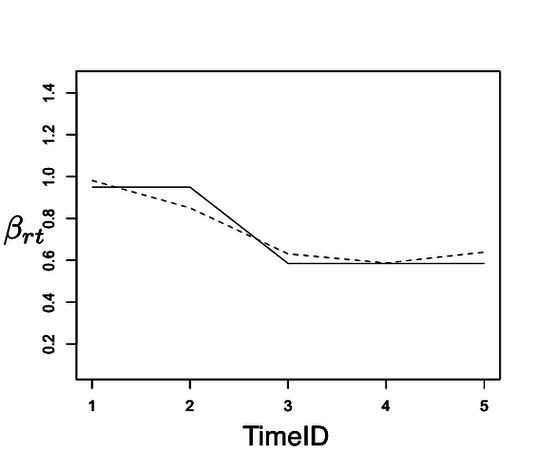
\includegraphics[keepaspectratio, scale=0.22]{img/beta_rt_param.png}
   % \subcaption{シミュレーション実験の結果例}
  \end{minipage}
  \begin{minipage}[b]{4cm}
    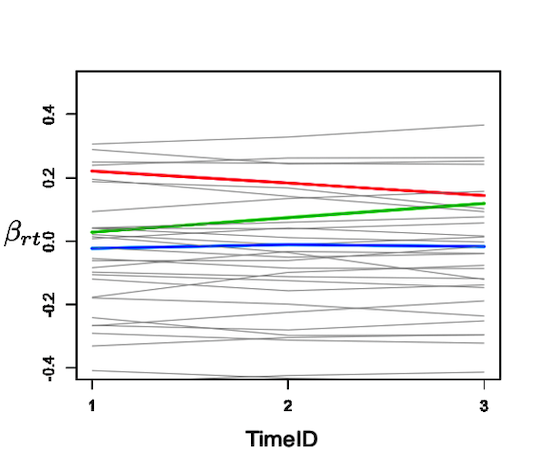
\includegraphics[keepaspectratio, scale=0.22]{img/beta_rt_data.png}
   % \subcaption{実データ実験の結果}
  \end{minipage}
 %  \vspace*{0.5cm}
  \caption{$\beta_{rt}$の推定結果の例}
  \label{beta_rt_data}
  \vspace*{0.5cm}
\end{figure}

また,提案モデルの性能を評価するために,情報量規準によるモデル比較を行った.ここでは, MCMCにより各モデルのパラメータを推定し,得られた推定値を用いて情報量規準を求めた.情報量規準にはMCMCのパラメータサンプルから算出できるWAIC(Widely Applicable Information Criterion)とWBIC(Widely Applicable Bayesian Information Criterion)を用いた.WAICは将来のデータの予測に優れたモデルを選択する規準である.他方で,WBICは真のモデルを漸近的に選択できる規準である.どちらの場合も,値が小さい方が適したモデルであることを示す.

時間区分数を$T=3$,$5$,$10$と変えて実験した結果を表\ref{WAICWBIC}に示す.
表\ref{WAICWBIC}から,各時間区分数におけるWAICとWBICの最小値を比較すると,提案モデルが最適モデルとして選択されたことが確認できる.

\begin{table}[t]
  \centering
  \begin{minipage}[t]{9cm}
    \centering
    \caption{モデル比較の結果}
    \setlength{\tabcolsep}{5.pt}
    \scalebox{0.8}{
      \begin{tabular}{cccccccc}  
        \bhline{1pt}
        &時間区分数  &既存モデル & 提案モデル \\ 
        \bhline{1pt}
        WAIC &3    & 3106.633 & \textbf{2956.466} \\
        &5    & 3171.920 & \textbf{2962.159} \\
        &10   & 3296.762 & \textbf{2961.461} \\
        \bhline{1pt}
        WBIC&3    & 1825.648 & \textbf{1808.674} \\
        &5    & 1916.035 & \textbf{1807.423} \\
        &10   & 2016.664 & \textbf{1806.655} \\
        \bhline{1pt}
      \end{tabular}
    }
    \label{WAICWBIC}
  \end{minipage}
\end{table}

\section{まとめと今後の課題}
本研究では,評価者の厳しさパラメータの時間変化にマルコフ性を仮定した新しい項目反応モデルを提案した.また,シミュレーション実験と実データを用いた実験を通して,提案モデルの有効性を示した.
今後の課題として,以下のものがある.
\begin{itemize}
  \item より大規模なデータを収集して,提案モデルの性能を評価する.
  \item 既存モデルと比べて提案モデルで採用した$\alpha_r$や$d_{rk}$の影響について分析を行う.
  \item 一般化多相ラッシュモデルのように,課題の特性も考慮できるように拡張を行う.
\end{itemize}

{\small
\bibliographystyle{chukan}
\bibliography{chukan}
}
\end{document}